\documentclass{article}

\usepackage{graphicx}
\usepackage{epstopdf}

\begin{document}

\section*{Matrices}
$M$ is a 121 x 24 matrix that takes a vector of function values on 24 coarse grid points to function values on 121 fine grid points on center square

$M = BA^{+}$ where B is a matrix that evaluates bessel functions on fine grid and A evaluates bessel functions on coarse grid 

$A$ is 24 x 17.
$B$ is 121 x 17

$A^{+} = V \Sigma_{n}^{+} U_{n}^{*}$ where $A = U_{n} \Sigma_{n} V^{*}$ is the thin SVD of A.


\section*{Figures}

\begin{figure}[h]
  \begin{center}
    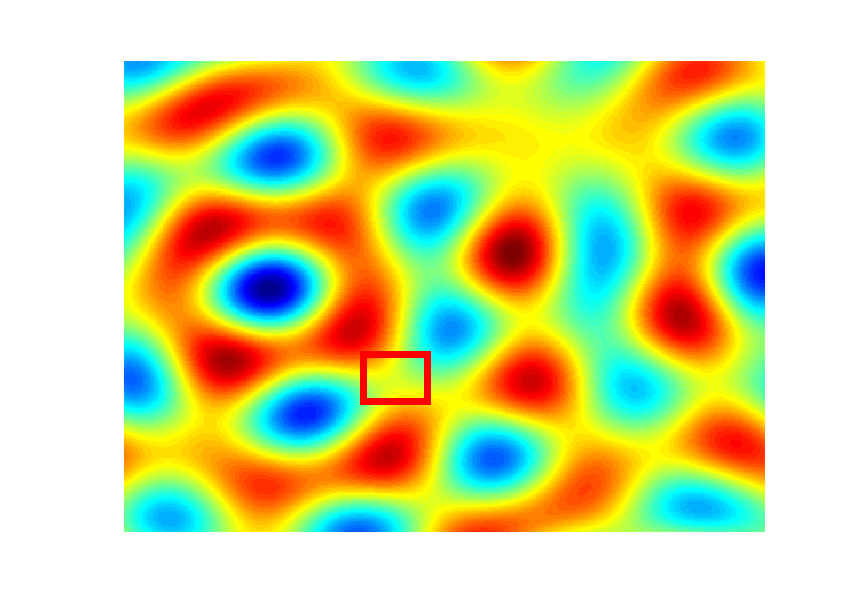
\includegraphics[width=0.75\textwidth]{figures/interpolation/high_res_rpw_with_rect.eps}
    \caption{A random combination of plane waves.}
  \end{center}
\end{figure}

\begin{figure}[h]
  \begin{center}
    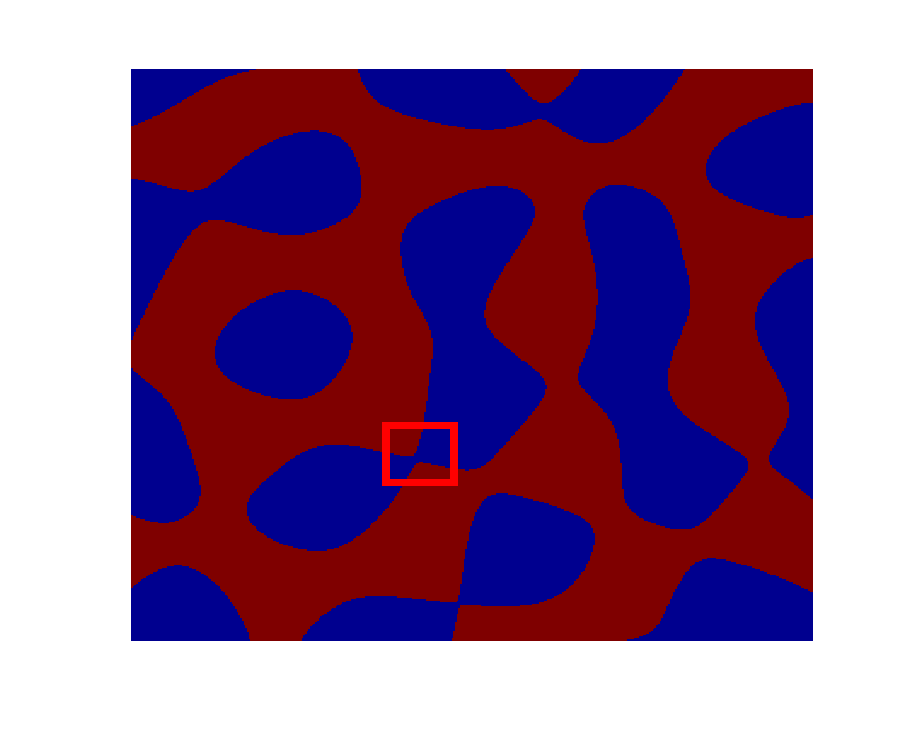
\includegraphics[width=0.75\textwidth]{figures/interpolation/high_res_domains_with_rect.eps}
    \caption{Nodal domains of the above RPW.}
  \end{center}
\end{figure}


\begin{figure}[h]
  \begin{center}
    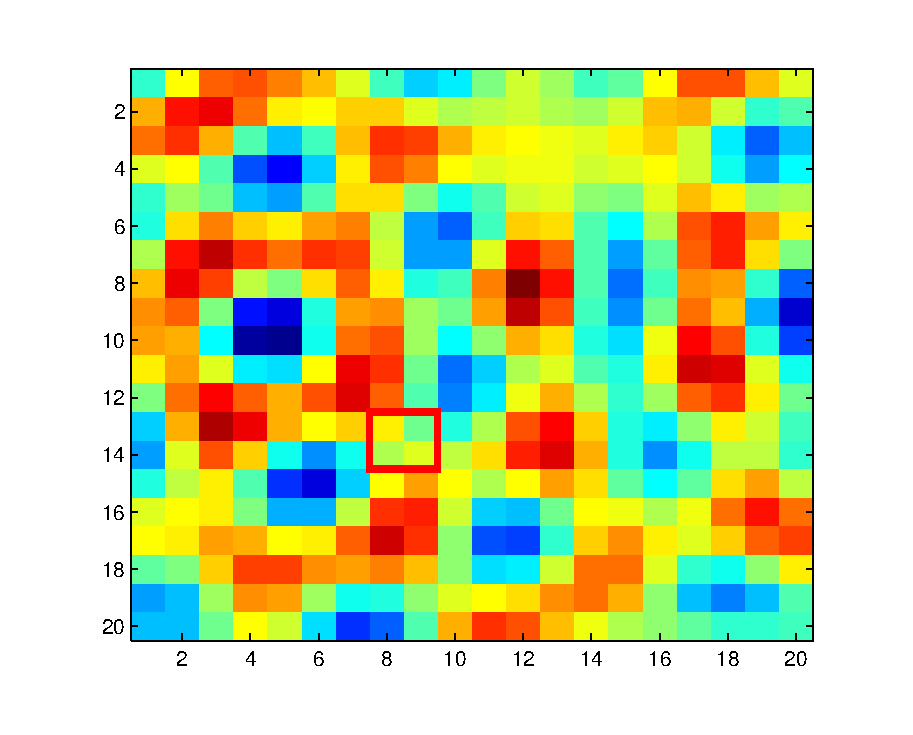
\includegraphics[width=0.75\textwidth]{figures/interpolation/low_res_rpw_with_rect.eps}
    \caption{The same RPW downsampled by a factor of 20 (in each direction).}
  \end{center}
\end{figure}

\begin{figure}[h]
  \begin{center}
    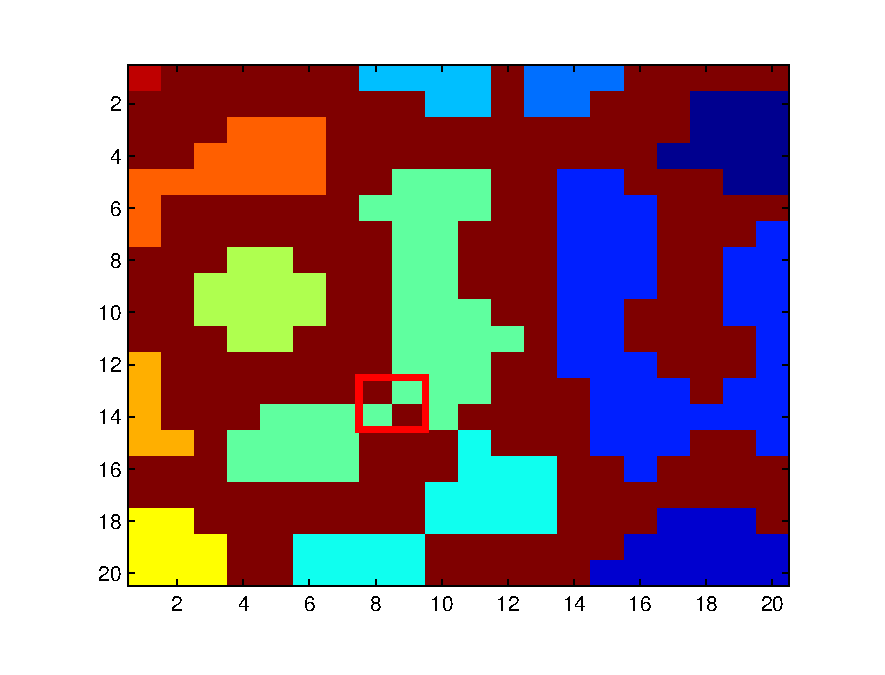
\includegraphics[width=0.75\textwidth]{figures/interpolation/low_res_domains_counted_with_rect.eps}
    \caption{Counted nodal domains of the downsampled RPW.}
  \end{center}
\end{figure}

\begin{figure}[h]
  \begin{center}
    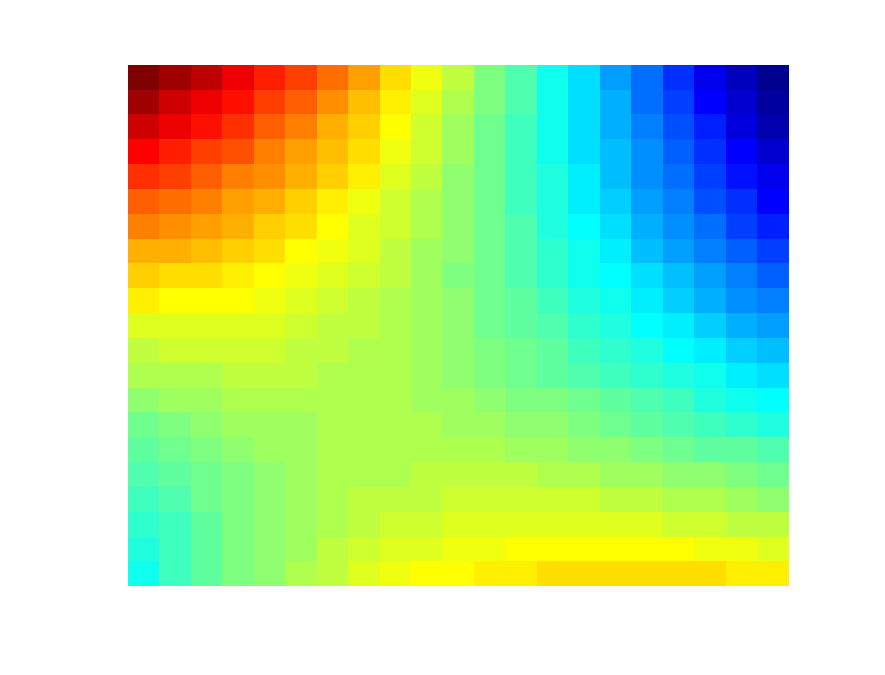
\includegraphics[width=0.75\textwidth]{figures/interpolation/high_res_trouble_spot_12_7.eps}
    \caption{Zoom of red rectangle in high resolution RPW.}
  \end{center}
\end{figure}

\begin{figure}[h]
  \begin{center}
    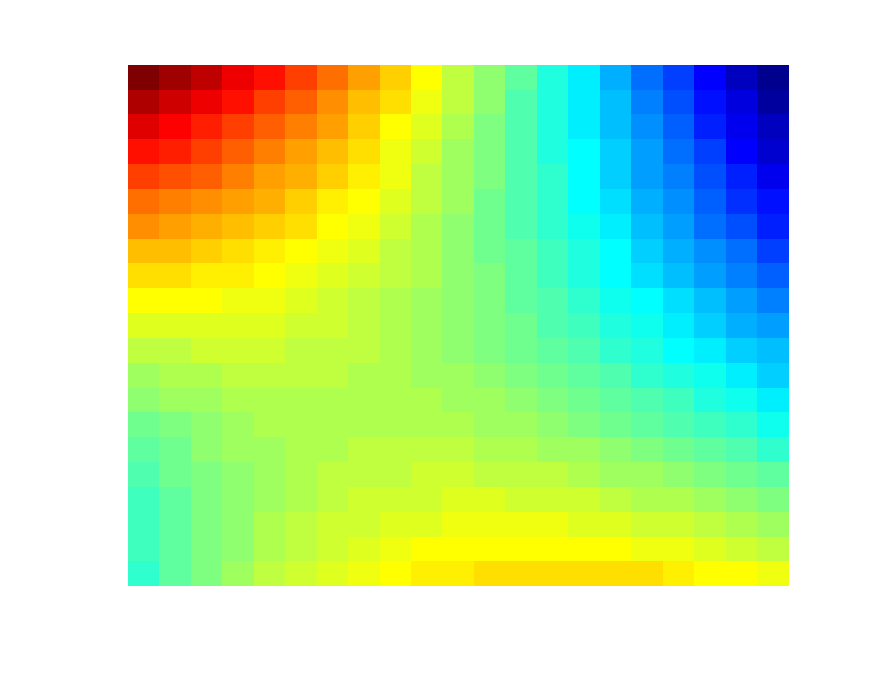
\includegraphics[width=0.75\textwidth]{figures/interpolation/interpolated_trouble_spot_12_7.eps}
    \caption{Result of interpolation in red rectangle.}
  \end{center}
\end{figure}


\end{document}
